% TRANSFORMATIONS, FUNCTIONS & EQUATIONS REVIEW - WORKSHEET 0 (IN-CLASS INSTRUCTION)
\documentclass[12pt, letterpaper, fleqn]{article}

% ----------------------------------------------------------
% PACKAGES
% ----------------------------------------------------------
\usepackage{graphicx}
\usepackage{xcolor}
\usepackage[most]{tcolorbox}
\usepackage{amsmath, amssymb}
\usepackage{fancyhdr}
\usepackage[utf8]{inputenc}
\usepackage[T1]{fontenc}
\usepackage{enumitem}
\usepackage{geometry}
\usepackage{tikz}
\usepackage{needspace}
\usepackage{multicol}

\usetikzlibrary{arrows.meta, calc, positioning}

% ----------------------------------------------------------
% PAGE SETUP
% ----------------------------------------------------------
\usepackage{times}
\geometry{letterpaper, top=1.25in, bottom=1.25in, marginpar=0.5in}

% ----------------------------------------------------------
% HEADER / FOOTER
% ----------------------------------------------------------
\newcommand{\logowidth}{3cm}
\setlength{\headheight}{20pt}
\setlength{\footskip}{40pt}

\pagestyle{fancy}
\fancyhf{}
\fancyhead[C]{\small\bfseries Transformations, Functions, and Equations Review}
\fancyfoot[L]{\raisebox{2pt}{
\includegraphics[width=\logowidth]{../kss.png}}}
\fancyfoot[C]{\thepage}
\fancyfoot[R]{8.24.0}

\renewcommand{\footrulewidth}{0.2pt}

% ----------------------------------------------------------
% THEME COLOR
% ----------------------------------------------------------
\definecolor{customteal}{HTML}{2fbdb9}

% ----------------------------------------------------------
% HELPER MACROS
% ----------------------------------------------------------
\newcommand{\blank}{\underline{\hspace{2.2cm}}}
\newcommand{\blanklong}{\underline{\hspace{6.5cm}}}
\newcommand{\blankshorter}{\underline{\hspace{1.5cm}}}

% ----------------------------------------------------------
% DOCUMENT
% ----------------------------------------------------------
\begin{document}

\textbf{Name:} \underline{\hspace{5cm}}
\hfill
\textbf{Date:} \underline{\hspace{3cm}}\\

% ==========================================================
% SECTION 1: FOUNDATION
% ==========================================================
\begin{tcolorbox}[colback=customteal!20]
    \large\textcolor{black}{\textbf{Foundation: Core Concepts Review}}
\end{tcolorbox}

\vspace{3mm}

\noindent
This unit reviews three major pillars of 8th grade math. Let's refresh our memory on the key rules for each.

\begin{itemize}
    \item \textbf{Transformations:} 
    \begin{itemize}
        \item \textbf{Translation:} Slide. $(x, y) \rightarrow (x+a, y+b)$.
        \item \textbf{Reflection:} Flip across an axis.
        \item \textbf{Rotation:} Turn around the origin.
        \item \textbf{Dilation:} Resize by a scale factor $k$. $(x, y) \rightarrow (kx, ky)$.
    \end{itemize}
    \item \textbf{Functions:} Every input $x$ has exactly ONE output $y$. Graphs must pass the Vertical Line Test.
    \item \textbf{Equations ($y = mx + b$):} The slope $m$ is the constant rate of change ($\text{rise}/\text{run}$). The $y$-intercept $b$ is the starting point on the $y$-axis.
\end{itemize}

\vspace{4mm}

% ==========================================================
% VISUAL REPRESENTATION
% ==========================================================
\begin{tcolorbox}[colback=white, colframe=black!25, boxrule=0.6pt, arc=4mm, left=6mm, right=6mm, top=5mm, bottom=5mm]

\textbf{Visual Representation: The Coordinate Plane Connections}

\medskip

\begin{center}
\begin{tikzpicture}[scale=0.8]
% Grid
\draw[step=1cm,gray!30,very thin] (-3,-3) grid (5,5);
\draw[thick,->] (-3.5,0) -- (5.5,0) node[right] {$x$};
\draw[thick,->] (0,-3.5) -- (0,5.5) node[above] {$y$};

% Line y = 2x - 1
\draw[thick, blue, <->] (-1, -3) -- (3, 5) node[right] {$y = 2x - 1$};
\filldraw[blue] (0,-1) circle (2.5pt) node[right, black] {$b = -1$};

% Function Mapping Visual (Abstract)
\node[draw, rounded corners, fill=red!10, text width=2cm, align=center] at (-2, 3) {\textbf{Function Test:}\\Passes!};
\draw[dashed, red, thick] (1.5, 4) -- (1.5, -2);
\node[red, font=\footnotesize] at (1.5, -2.3) {Vertical Line};

\end{tikzpicture}
\end{center}

\medskip
\begin{itemize}
    \item The line $y = 2x - 1$ is a \textbf{linear equation}.
    \item It is a \textbf{function} because any vertical line (like the red dashed line) only crosses the blue line once.
    \item If we applied a \textbf{translation} to slide this line UP by 3 units, the new $y$-intercept would be $b=2$, and the new equation would be $y = 2x + 2$.
\end{itemize}

\end{tcolorbox}

\vspace{4mm}

\newpage

% ==========================================================
% WORKED EXAMPLES
% ==========================================================
\begin{tcolorbox}[colback=customteal!20]
\large\textcolor{black}{\textbf{Reviewing Equation Solving}}
\end{tcolorbox}

\vspace{3mm}

\begin{tcolorbox}[colback=white, colframe=black!25, boxrule=0.6pt, arc=4mm, left=6mm, right=6mm, top=5mm, bottom=5mm]

\textbf{Worked Example 1: Solving Multi-Step Equations}

\medskip

\textbf{Problem:} Solve for $x$: \ \ $3(x - 2) + 4 = 5x - 8$

\medskip

\textbf{Solution:}
\begin{itemize}
    \item \textbf{Step 1 (Distribute):} \ \ $3x - 6 + 4 = 5x - 8$
    \item \textbf{Step 2 (Combine Like Terms):} \ \ $3x - 2 = 5x - 8$
    \item \textbf{Step 3 (Move Variables):} Subtract $3x$ from both sides.
    \[ -2 = 2x - 8 \]
    \item \textbf{Step 4 (Move Constants):} Add $8$ to both sides.
    \[ 6 = 2x \]
    \item \textbf{Step 5 (Isolate):} Divide by $2$. \ \ $x = 3$.
\end{itemize}

\end{tcolorbox}

\vspace{4mm}

% ==========================================================
% PRACTICE 1
% ==========================================================
\begin{tcolorbox}[colback=white!15, colframe=black, boxrule=1.5pt, arc=4mm, left=6mm, right=6mm, top=5mm, bottom=5mm]

\textbf{Guided Practice: Concept Checks}

\medskip

\noindent
\textbf{1.} Point $A(2, 5)$ is reflected across the $x$-axis. What are the coordinates of $A'$?
\vspace{1cm}

\noindent
\textbf{2.} Write the equation of a line passing through $(0, 4)$ with a slope of $-\dfrac{1}{2}$.
\vspace{1.5cm}

\noindent
\textbf{3.} Does the table below represent a function? Why or why not?

\begin{tabular}{|c|c|c|c|c|}
\hline
$x$ & 3 & 4 & 5 & 3 \\
\hline
$y$ & 7 & 8 & 9 & 10 \\
\hline
\end{tabular}

\vspace{1.5cm}

\end{tcolorbox}

\newpage

% ==========================================================
% THINKING PROBLEM
% ==========================================================
\begin{tcolorbox}[colback=customteal!20]
\large\textcolor{black}{\textbf{Deeper Thinking: Pulling It All Together}}
\end{tcolorbox}

\vspace{3mm}

\begin{tcolorbox}[colback=white!15, colframe=black, boxrule=1.5pt, arc=4mm, left=6mm, right=6mm, top=5mm, bottom=5mm]

\textbf{Deeper Thinking Problem 1: The Triangle Translation}

\medskip

\noindent
A triangle is defined by the following points: $X(1, 2), Y(4, 2), \text{ and } Z(1, 6)$.

\vspace{5mm}

\noindent
\textbf{a)} Draw this triangle on a coordinate plane. Find the length of the horizontal leg $XY$ and the vertical leg $XZ$.

\vspace{2.5cm}

\noindent
\textbf{b)} Use the Pythagorean theorem to find the length of the hypotenuse $YZ$.

\vspace{2.5cm}

\noindent
\textbf{c)} Now, translate the entire triangle left $3$ units and down $4$ units. Write the new coordinates for $X', Y', \text{ and } Z'$.

\vspace{2.5cm}

\noindent
\textbf{d)} Did the length of the hypotenuse $Y'Z'$ change during this translation? Why or why not? What do we call this type of transformation?

\vspace{2cm}

\end{tcolorbox}

\end{document}
